\section{Related Work}

\subsection{Previous work by the NDN team}

This network environment continues work that began in the original NDN project on authenticated lighting control and was extended through an EAGER in 2012-2013 to explore sensing and building management.  The current and ongoing research, its results, and our evolving testbed are described in Section~\ref{sec:instrumented}.  

\subsection{Suggested reading}

Stouffer, Keith, Joe Falco, and Karen Scarfone. "Guide to industrial control systems (ICS) security." NIST Special Publication (2013): 800-82 Revision 1.

Shang, W., Ding, Q., Marianantoni, A., Burke, J., Zhang, L. “Securing Building Management System Using Named Data Networking.”  (to be 
released as a TR), 2013. 

Burke, J. Gasti, P., Nanthan, N., Tsudik, G. “Securing Instrumented Environments over Content-Centric Networking: the Case of Lighting Control.”  Proc. IEEE NOMEN, April 2013. 

Dawson-Haggerty, Stephen, et al. "BOSS: building operating system services." Proceedings of the 10th USENIX Symposium on Networked Systems Design and Implementation (NSDI). 2013.

\subsection{Building Operating System Services (BOSS)} 

\begin{figure}
\begin{center}
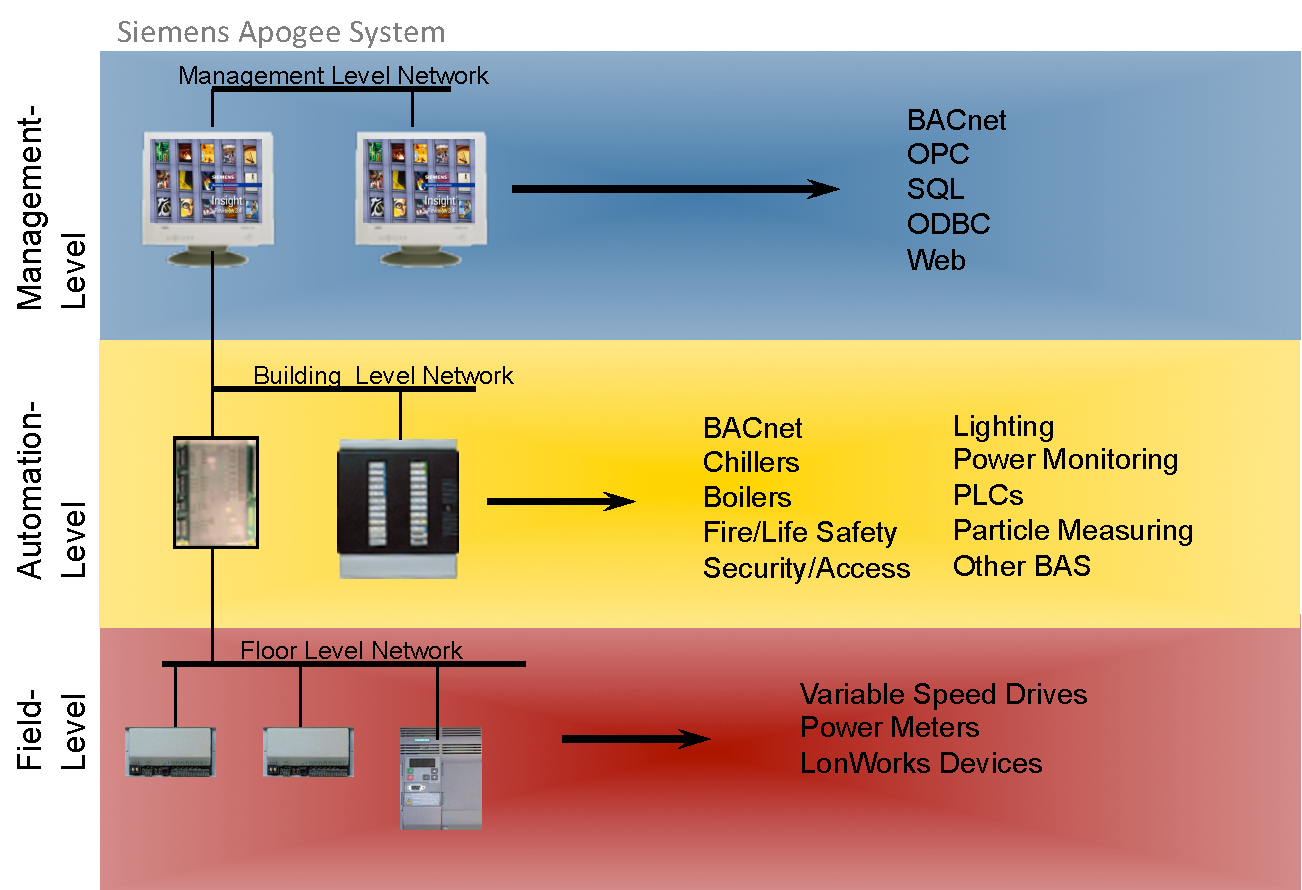
\includegraphics[width=.6\textwidth]{figures/siemens-apogee-levels}
\caption{Architecture of Building Operating System Services (BOSS) from UCB~\cite{Dawson-Haggerty2013BOSS}.} 
\label{fig:BOSS}
\end{center}
\end{figure}

Observation:  Existing buildings are not ``programmable" because there are no layers of abstraction for devices.  So, applications are not portable and access to building systems is not protected.

Proposal: Provide an ``operating system" to ``knit together existing pieces of infrastructure, Internet data feeds, and human feedback into a cohesive, extendable, and programmable system." 

Support multiple, fault-tolerant applications running on top of the distributed physical resources in large commercial buildings. 

Six subsystems:
\begin{enumerate}
\item Hardware and access abstractions;
\item Naming and semantic modeling;
\item Real-time time series processing and archiving;
\item Control transaction system;
\item Authorization;
\item Running applications.
\end{enumerate}

See Figure~\ref{fig:BOSS} for their relationship. 